\chapter{Relation Between Dielectric Properties and Structure in Complex Amorphous and Crystalline Thin Film Oxides}

This chapter is adapted from T. A. Naoi and R. B. van Dover: ``Relation Between Dielectric Properties and Structure in Complex Amorphous and Crystalline Thin Film Oxides'' in preparation.

% ABSTRACT
\section{Abstract}
We have used off-axis magnetron sputtering to explore changes in the structural and dielectric properties of pseudo-ternary thin film dielectrics as a function of composition. We investigated four different oxide systems: (HfO$_{2}$)$_{1-x}$(SiO$_{2}$)$_{x}$, (HfO$_{2}$)$_{1-x}$(GeO$_{2}$)$_{x}$, (Nb$_{2}$O$_{5}$)$_{1-x}$(GeO$_{2}$)$_{x}$, and (Ta$_{2}$O$_{5}$)$_{1-x}$(SnO$_{2}$)$_{x}$. The diffraction patterns of (HfO$_{2}$)$_{1-x}$(SiO$_{2}$)$_{x}$ and (HfO$_{2}$)$_{1-x}$(GeO$_{2}$)$_{x}$ were highly similar, where the onset of crystallinity was slightly higher for HfO$_{2}$ films doped with SiO$_{2}$. However, the similarity in diffraction pattern does not translate into comparable dielectric behavior. We obtain a maximum dielectric constant of $\varepsilon_{r} = 28$ at 96 at$\%$ Hf for (HfO$_{2}$)$_{1-x}$(SiO$_{2}$)$_{x}$ whereas for (HfO$_{2}$)$_{1-x}$(GeO$_{2}$)$_{x}$ $\varepsilon_{r}$ is only 19. The refractive indices vary linearly with composition for both systems. (Ta$_{2}$O$_{5}$)$_{1-x}$(SnO$_{2}$)$_{x}$ was crystalline only for the most Ta poor regions and remained amorphous for Ta cation fractions greater than 15$\%$. Dielectric dispersion increased with increasing SnO$_{2}$ composition, which we assume is a result of defect and interstitial mediated conduction in SnO$_{2}$. Finally, anomalous features in the dielectric constant and refractive index were not evident in (Nb$_{2}$O$_{5}$)$_{1-x}$(GeO$_{2}$)$_{x}$. It is possible to obtain a high quality dielectric by doping low levels of GeO$_{2}$ into Nb$_{2}$O$_{5}$ and may be useful for applications requiring an amorphous oxide with a high dielectric constant.
    
\section{INTRODUCTION} 
The wide application of thin film oxides is a testament to its importance in modern technology. They are used in optical coatings, \cite{Cevro1995} photocatalysis, \cite{Fujishima1972} gate oxides, \cite{Wilk2000a} and capacitors \cite{Kim2008}. A relatively straightforward way to improve capacitor performance is to increase the dielectric constant of the insulator, $\varepsilon_{r}$, which can be achieved by stabilizing a high $\varepsilon_{r}$ crystal structure by selective doping. \cite{Govindarajan2007, Chalker2008, TsouTsou2009, Tomida2006} Crystallization of the material is not necessarily deleterious, but in some applications we would like to prevent the materials from crystallizing. Thus, it would be desirable to enhance $\varepsilon_{r}$ without inducing substantial crystallization. This effect has been observed for example, in hafnium and zirconium silicates with some controversy. \cite{Wilk2000a, Lucovsky2000, Pignedoli2007} It may well be that the effects were real, but the disordered nature of these materials makes it difficult to understand the origin of these outstanding properties, so that the results can be replicated through tailored processing. Enhanced amorphous dielectric properties have also been observed experimentally in tantalum and niobium based oxides, such as (Ta$_{1-x}$Nb$_{x}$)$_{2}$O$_{5}$ and (Ta$_{2}$O$_{5}$)$_{1-x}$(GeO$_{2}$)$_{x}$ solid solutions. \cite{Kukli1999,Naoi2012} In the case of (Ta$_{1-x}$Nb$_{x}$)$_{2}$O$_{5}$, the dielectric constant jumped to $\varepsilon_{r} = 33$ at a Nb/(Nb+Ta) ratio of 42\%, though the leakage current was markedly higher, and niobium oxide has a higher $\varepsilon_{r}$ to begin with in comparison to tantala. \cite{Kukli1999} For (Ta$_{2}$O$_{5}$)$_{1-x}$(GeO$_{2}$)$_{x}$, the dielectric constant rose to $\varepsilon_{r} \sim 33$, strangely at a composition that is least GeO$_{2}$ rich. \cite{Naoi2012} Introduction of SiO$_{2}$ on the other hand does not induce such effect. \cite{Naoi2018jap}

The drastic differences in behavior even between materials doped with chemically similar oxides in itself is intriguing, and hence worth exploring. In this study, we examine the composition dependent dielectric and structural properties of (HfO$_{2}$)$_{1-x}$(SiO$_{2}$)$_{x}$, (HfO$_{2}$)$_{1-x}$(GeO$_{2}$)$_{x}$, (Nb$_{2}$O$_{5}$)$_{1-x}$(GeO$_{2}$)$_{x}$, and (Ta$_{2}$O$_{5}$)$_{1-x}$(SnO$_{2}$)$_{x}$ using off-axis reactive magnetron cosputtering. (HfO$_{2}$)$_{1-x}$(SiO$_{2}$)$_{x}$ is a system that has been studied heavily, whereas (HfO$_{2}$)$_{1-x}$(GeO$_{2}$)$_{x}$ has garnered considerably less attention. We expect the two systems to behave similarly, owing to the chemical similarities between SiO$_{2}$ and GeO$_{2}$. Likewise, one would expect some similarity in the composition dependence of the dielectric properties of (Nb$_{2}$O$_{5}$)$_{1-x}$(GeO$_{2}$)$_{x}$, (Ta$_{2}$O$_{5}$)$_{1-x}$(GeO$_{2}$)$_{x}$, and  (Ta$_{2}$O$_{5}$)$_{1-x}$(SnO$_{2}$)$_{x}$. Crystalline Nb$_{2}$O$_{5}$ tends to be a leaky oxide due to grain boundary conduction, which can be mitigated by forming an amorphous oxide to eliminate grain boundaries, or selective doping. \cite{Pignolet1995,Kukli1999} The properties of  (Ta$_{2}$O$_{5}$)$_{1-x}$(SnO$_{2}$)$_{x}$ have been characterized, but the composition resolution is low and the study was focused on Sn rich compositions, whereas the effect seen in (Ta$_{2}$O$_{5}$)$_{1-x}$(GeO$_{2}$)$_{x}$ occurs for GeO$_{2}$ rich compositions. \cite{Fujikawa1997}

\section{EXPERIMENTAL METHODS}

%Sputtering
We fabricated the binary oxide compositions spreads in similar fashion to previously published experiments. \cite{Vandover1998} Films were sputtered on to 3 in. Si wafers precoated with e-beam evaporated 300 \AA\ Cr and 350 \AA\ Pt. Prior to film deposition the chamber was evacuated to a pressure of 10$^{-6}$ Torr. The deposition condition for all films is summarized in Table \ref{tab:depcond}.

\begin{table}[h]
\centering
\caption{Deposition conditions for films sputtered in this experiment.}
\begin{tabular}{lccccc}
\hline\hline
Oxide System & Power(W) & Gas & FlowRate(sccm) & Pressure\\
\hline
Hf-Si-O & 100-20 & Ar/O$_{2}$ & 15/10 & 30mTorr\\
Hf-Ge-O & 100-20 & Ar/O$_{2}$ & 15/10 & 30mTorr\\
Nb-Ge-O & 100-20 & Ar/O$_{2}$ & 15/10 & 30mTorr\\
Ta-Sn-O & 100-30 & Ar/O$_{2}$ & 15/10 & 30mTorr\\ \hline
\end{tabular}
\label{tab:depcond}
\end{table}

\noindent The substrate was also intentionally biased at -75 V to ensure the formation of a dense film. Applying a substrate bias precludes the formation of columnar voids during deposition \cite{Barron2009}, which is undesirable when characterizing intrinsic film characteristics. Substrate temperature during deposition was below 60\textcelsius. 

%X-ray diffraction
A Bruker General Area Detector Diffraction System (GADDS) was used to collect X-ray diffraction intensities at several points on the wafer. Standard Cu-K$\alpha$ x-rays  ($\lambda = 1.5418$ \AA) were used at 40kV and 40mA. The advantage of GADDS is the two-dimensional area detector which can captures a larger portion of the diffraction ring, otherwise not possible using a conventional diffractometer that is confined within a diffraction plane. We oriented the sample such that the captured image represents diffraction patterns corresponding to $2\theta$ from roughly 20-70\textdegree. The detector position was fixed at $2\theta = 40$\textdegree, while $\omega = 20$\textdegree\ and $\phi = 0$\textdegree. Collection time was limited to 300 seconds achieving a high signal to noise ratio. The captured intensity was post-processed and integrated azimuthally in $\chi$ to generate a powder diffraction pattern.    

%XRR
We determined the film density by x-ray reflectivity (XRR) using a Rigaku Smartlab x-ray diffractometer as previously reported elsewhere. \cite{Naoi2018jap} Briefly, Cu K$\alpha$ X-rays at 40mA/44kV were conditioned through x-ray optics. In this experiment we used a Ge-002 crystal monochrometer for improved accuracy. 1-D scans were conducted across the wafer at 21 equally spaced points along the long axis. At each point, scans were taken in the $\theta$ - 2$\theta$ geometry by varying the incident angle. Based on the x-ray beam footprint, we estimate the maximum error in composition for the density measurement to be roughly $\pm$5$\%$, though depending on the measured point the error was typically much smaller. Film density was directly evaluated by first determining critical angle $\theta_{c}$ \cite{Parratt1954} and using the following,
\begin{equation}
\rho = \frac{\theta_{c}^{2}\pi A}{Zr_{e}\lambda^{2} N_{A}} 
\end{equation}
where A is the atomic mass unit, $r_{e}$ classical electron radius, $\lambda$ the wavelength of the x-ray, $N_{A}$ is Avogadro’s number, and Z the atomic number. We estimate the composition using previously determined deposition rates. 


%Ellipsometry
Index of refraction and film thickness were determined using a J.A. Woollam Variable Angle Spectroscopic Ellipsometer. The ellipsometric parameters $\psi$ and $\delta$ were measured at 65, 70, and 75\textdegree. At each angle the wavelength was varied from 450 - 1000 nm at 100 nm increments. A film/substrate bilayer model was used to fit $\psi$ and $\delta$. The optical constants of the substrate layer was determined prior to film deposition and was fixed during the fitting process. The film was modeled using a two-term Cauchy relation, $n(\lambda) =  A + \frac{B}{\lambda^{2}}$. The WVASE32 software package supplied by J.A. Woollam was used to fit $A$, $B$, and thickness by recursively varying the parameters to minimize the mean squared error. The refractive index was taken to be A, which is the refractive index at the infinite wavelength limit well away from absorption edge.

%LCR measurements
Electrical characterization was performed by preparing a metal-insulator-metal structure (MIM). Top electrodes (200 micron diameter, 350 \AA\ thick) were electron beam evaporated on to the film through a shadow mask. Contact to the top electrode was made using a BeCu tip while gold wire was soldered to the bottom electrode using indium solder. Capacitance and $\tan\delta$, i.e. $\frac{Re(\epsilon)}{Im(\epsilon)}$, was measured across the MIM capacitor using a HP 4284 precision inductance-capacitance-resistance (LCR) meter at 100 mV over the frequency range of 100 Hz - 100 kHz. 

\section{RESULTS AND DISCUSSION} 

\subsection{(HfO$_{2}$)$_{1-x}$(SiO$_{2}$)$_{x}$ and (HfO$_{2}$)$_{1-x}$(GeO$_{2}$)$_{x}$}

We first present the results for the diffraction measurements. The strong reflections at roughly 2$\theta =$ 39.5\textdegree, 46\textdegree, and 67\textdegree observed in all samples correspond to the (111), (200), and (220) diffraction planes respectively generated by the Pt bottom electrode. Additionally, the recurring peaks at 44$^{\circ}$ corresponds to the Cr (110) underlayer, while the peak at 34$^{\circ}$ is a detector artifact. 

\begin{figure}
\centering
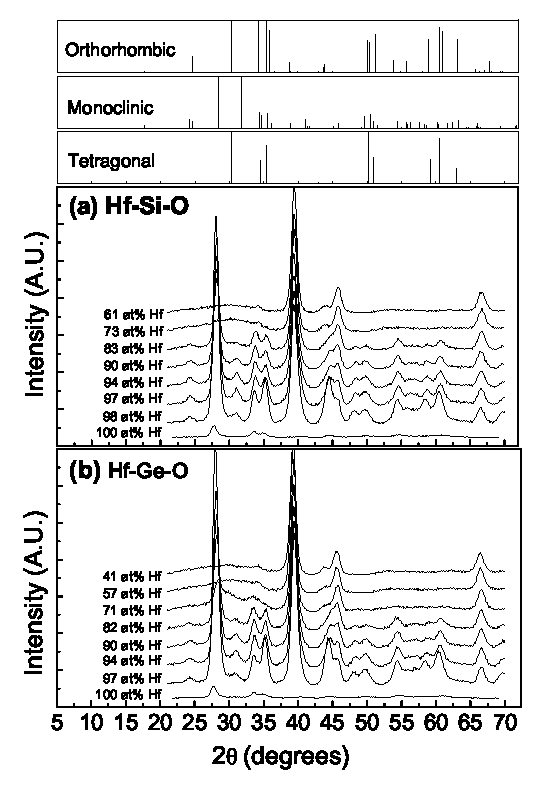
\includegraphics[width=0.5\linewidth]{chapter_6/hfsigeox_wpdf.eps}
\caption{The XRD spectra for (a) (HfO$_{2}$)$_{1-x}$(SiO$_{2}$)$_{x}$ and (b) (HfO$_{2}$)$_{1-x}$(GeO$_{2}$)$_{x}$ plotted for several different Hf cation compositions. The observed patterns between Si and Ge doped HfO$_{2}$ are highly similar, demonstrating their chemical resemblance. The diffraction pattern for the mixed films show that the monoclinic phase is the dominant phase, however comparison with available diffraction patterns suggest the presence of other metastable phases. For reference the diffraction pattern of pure HfO$_{2}$ is shown at the bottom. The weak reflections reveal the presence of partially crystalline domains.}  
\label{fig:xrd1}
\end{figure}

For the hafnium based systems a change in composition elicits a clear shift in the structure from amorphous (HfO$_{2}$ poor compositions) to polycrystalline (HfO$_{2}$ rich compositions), as seen in Figure \ref{fig:xrd1}. As a reference we also present the diffraction pattern of pure HfO$_{2}$ deposited under similar conditions. The pattern displays very weak reflections signifying the presence of small crystalline domains embedded in a mostly disordered matrix. 

It is not unusual that the doped hafnia films deposited at low temperatures show sign of crystallinity. Thicker HfO$_{2}$ films may crystallize \cite{Ritala1994} (our films are 100 - 300 nm thick) and deposition conditions \cite{Jones1992, Wang2008} play a role in whether HfO$_{2}$ becomes amorphous or crystalline. Even for films that seem to be amorphous HfO$_{2}$ thin films, careful inspection of its structure reveals that it exhibits a certain level of medium-range order, a characteristic of a fairly poor glass former. \cite{Ho2003} Crystallinity decreases with increasing substitution of glass formers SiO$_{2}$ and GeO$_{2}$ and is consistent with our intuition that substitution of glass formers should increase the crystallization temperature of the film. \cite{Maria2002}

A direct comparison of the diffraction patterns between the two systems shows an uncanny resemblance, demonstrating the chemical similarities between SiO$_{2}$ and GeO$_{2}$. Continuous rings are observed in the area detector pattern, which indicate that the grains are equiaxed with no preferential orientation. Comparison with powder diffraction and calculated diffraction patterns retrieved from the Inorganic Crystal Structure Database (ICSD) with the integrated powder diffraction patterns show that the HfO$_{2}$ rich crystalline films primarily consist of the monoclinic phase, indicated definitively by the peak at 28.2$^{\circ}$. Note, the bulk equilibrium phase of HfO$_{2}$ at room temperature is monoclinic. 

\begin{figure}
\centering
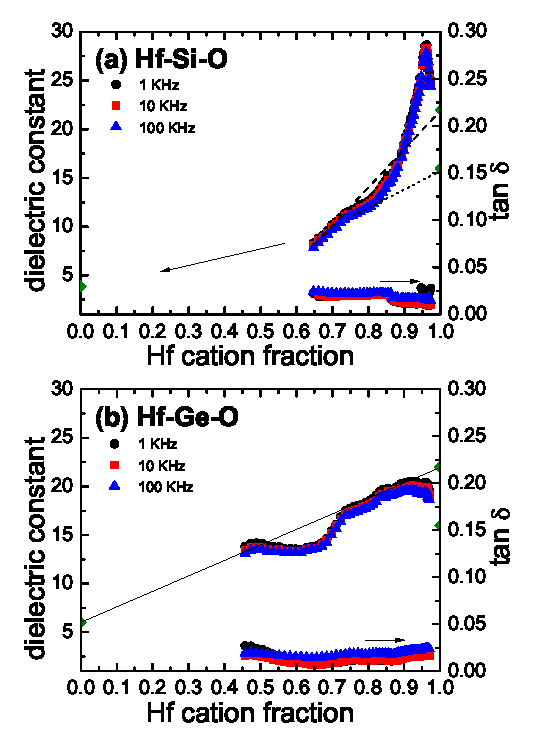
\includegraphics[width=0.5\linewidth]{chapter_6/eps_hfsigeox.eps}
\caption{The dielectric constant and dissipation factor of (a) (HfO$_{2}$)$_{1-x}$(SiO$_{2}$)$_{x}$ and (b) (HfO$_{2}$)$_{1-x}$(GeO$_{2}$)$_{x}$ as function of Hf cation composition. In contrast to the XRD patterns in Figure \ref{fig:xrd1}, the dielectric behavior of the two materials are different.}
\label{fig:eps1}
\end{figure} 

However, we see the peaks are not well aligned with a pure monoclinic phase. The structural deviation is reflected in the dielectric behavior of the two systems as a function of composition (Figure \ref{fig:eps1}). For (HfO$_{2}$)$_{1-x}$(SiO$_{2}$)$_{x}$, we see that a rough extrapolation of $\varepsilon_{r}$ to pure SiO$_{2}$ in the amorphous region ($65 < \text{at\% Hf} < 75$) points to about 3.9. A linear extrapolation in the other direction to pure HfO$_{2}$ (denoted by the dashed line) yields $\varepsilon_{r}$ of 22, the dielectric constant of pure amorphous HfO$_{2}$. \cite{Ceresoli2006} At the onset of crystallization in the region $75 < \text{at\% Hf} < 85$, we observe a slope change in $\varepsilon_{r}$ (dotted line) such that now $\varepsilon_{r}$ extrapolates to the dielectric constant of monoclinic HfO$_{2}$, $\varepsilon_{r} = 16$. \cite{Zhao2002} Further addition of HfO$_{2}$ causes another slope change at $\sim$85 at\% Hf accompanied by a discontinuity in tan $\delta$. In this region $\varepsilon_{r}$ is enhanced dramatically to a maximum dielectric constant of approximately 28 at a concentration of 96 at\% Hf. The dielectric behavior in this region is clear indication that the monoclinic phase is not the sole phase within this composition range, since $\varepsilon_{r}$ of a pure monoclinic phase is only 16. Finally, the dielectric constant drops down for even higher Hf concentrations.

The dielectric behavior of (HfO$_{2}$)$_{1-x}$(GeO$_{ 2}$)$_{x}$ is clearly different from (HfO$_{2}$)$_{1-x}$(SiO$_{ 2}$)$_{x}$, even though their diffraction patterns are highly similar. At 50 $  \text{at\% Hf}$, the dielectric constant is consistent with the linear interpolation (solid line), between the endmember values for pure amorphous HfO$_{2}$ and GeO$_{2}$. Addition of Hf does not increase the dielectric constant and consequently, $\varepsilon_{r}$ is suppressed below the linear interpolation for $50 < \text{at\% Hf} < 70$. At the onset of crystallization ($\sim$70 at\% Hf) the dielectric constant once again becomes collinear to the linear interpolation. Increasing the Hf concentration further does not result in any kind of enhancement; the dielectric constant of the Hf richest composition is 19, roughly between the amorphous and monoclinic dielectric constant. 

Without further analysis, it is difficult to determine the cause for the trends seen in Figure \ref{fig:eps1}. Nevertheless, the enhancement of $\varepsilon_{r}$ observed in (HfO$_{2}$)$_{1-x}$(SiO$_{ 2}$)$_{x}$ is unfeasible without a stabilization of high $\varepsilon_{r}$ phases such as the tetragonal, or cubic like phase. It has been shown that both Si and Ge are effective stabilizers of the tetragonal phase, where Si is slightly more effective than Ge, i.e. lower concentrations of the dopant is required. \cite{Fischer2008a, Tomida2006} Its effectiveness in part may be attributed to ionic radii where smaller dopants such as Si and Ge tend to stabilize the tetragonal phase. \cite{Lee2008} For stabilization of the tetragonal phase, calculations by Lee et al. \cite{Lee2008}  predict a minimum concentration of 10.9\% for Si and 18.6 \% for Ge. Furthermore, when considering temperature as a parameter,  Debernardi predicts that at 320 K, 12.5\% Ge is required to stabilize the tetragonal phase. \cite{Debernardi2012} Our data suggests that it is fairly easy to stabilize a tetragonal-like phase when Si is the dopant, while Ge seems less effective and may require additional processing. Deviations from predicted values may be caused by stress and grain size effects, which shift the transformation temperature. \cite{Garvie1978} It is possible that the deposition process and the dopant in combination have created stresses in the film causing the variations.

\begin{figure}
\centering
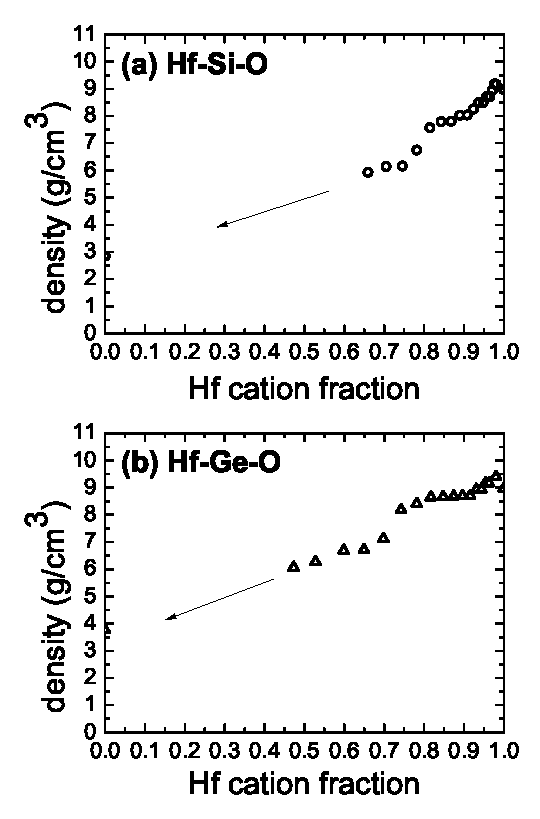
\includegraphics[width=0.5\linewidth]{chapter_6/hfsiox_density.eps}
\caption{The density of (a) (HfO$_{2}$)$_{1-x}$(SiO$_{2}$)$_{x}$ and (b) (HfO$_{2}$)$_{1-x}$(GeO$_{2}$)$_{x}$ as function of Hf cation composition determined using XRR. Crystallization of the film causes the film density to jump dramatically.}
\label{fig:hfd1}
\end{figure}

\begin{figure}
\centering
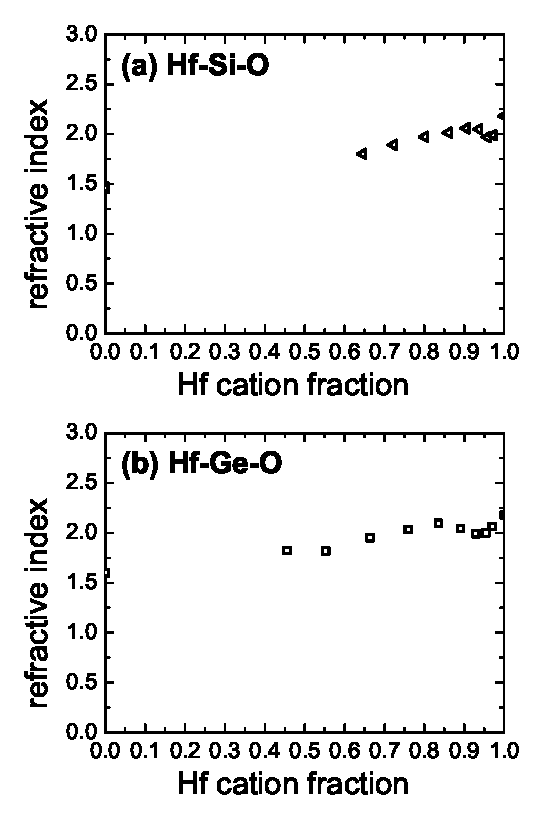
\includegraphics[width=0.5\linewidth]{chapter_6/n_hfsigeox.eps}
\caption{Refractive index of (a) (HfO$_{2}$)$_{1-x}$(SiO$_{2}$)$_{x}$ and (b) (HfO$_{2}$)$_{1-x}$(GeO$_{2}$)$_{x}$ as function of Hf cation composition.}
\label{fig:hfn1}
\end{figure}

We also present the density and the refractive indices in Figures \ref{fig:hfd1} and \ref{fig:hfn1} respectively as a function of Hf composition. The density for both systems increases linearly with increasing Hf composition in the amorphous regions. Crystallization of the film is marked by a clear jump in the density. The onset of crystallinity for (HfO$_{2}$)$_{1-x}$(GeO$_{2}$)$_{x}$ is slightly lower in composition in comparison to the (HfO$_{2}$)$_{1-x}$(SiO$_{2}$)$_{x}$; approximately 70 at\% Hf for Ge doped HfO$_{2}$ versus 80 at\% Hf for Si doping. This suggests the slightly higher effectiveness of SiO$_{2}$ as a glass former compared to GeO$_{2}$. We find that although there is a general correlation between increased density  and dielectric constant, there is no direct evidence which explains the large disparity in dielectric behavior between (HfO$_{2}$)$_{1-x}$(SiO$_{2}$)$_{x}$ and (HfO$_{2}$)$_{1-x}$(GeO$_{2}$)$_{x}$. For example, direct comparison of the density of both systems at around 96 at\% Hf, the density of (HfO$_{2}$)$_{1-x}$(SiO$_{2}$)$_{x}$ is 8.72 g/cm$^{3}$, whereas the density of (HfO$_{2}$)$_{1-x}$(GeO$_{2}$)$_{x}$ is 9.17 g/cm$^{3}$. This in turn implies that substantial differences in the phononic contributions may be at play.   

The refractive index varies linearly with Hf composition for both systems. For the Hf richest compositions a slight depression from a linear trend is observed. A large variation in the refractive index for HfO$_{2}$ is not uncommon, \cite{Jones1992} but a more likely contribution is the increase in roughness with crystallinity, \cite{Ritala1994} indicated by a larger mean squared error (MSE) in the fitting, as our simple model does not take into account surface roughness.  	
\subsection{(Nb$_{2}$O$_{5}$)$_{1-x}$(GeO$_{2}$)$_{x}$ and  (Ta$_{2}$O$_{5}$)$_{1-x}$(SnO$_{2}$)$_{x}$}

The XRD patterns for (Nb$_{2}$O$_{5}$)$_{1-x}$(GeO$_{2}$)$_{x}$ and  (Ta$_{2}$O$_{5}$)$_{1-x}$(SnO$_{2}$)$_{x}$ are shown in Figure \ref{fig:xrd2}. Patterns for (Nb$_{2}$O$_{5}$)$_{1-x}$(GeO$_{2}$)$_{x}$ show that it is amorphous for all compositions investigated, whereas crystallization is observed for tantalum poor compositions in (Ta$_{2}$O$_{5}$)$_{1-x}$(SnO$_{2}$)$_{x}$. Comparison with Power Diffraction File (PDF) suggest that the peaks embody the symmetry of the tetragonal (cassiterite) phase.

\begin{figure}
\centering
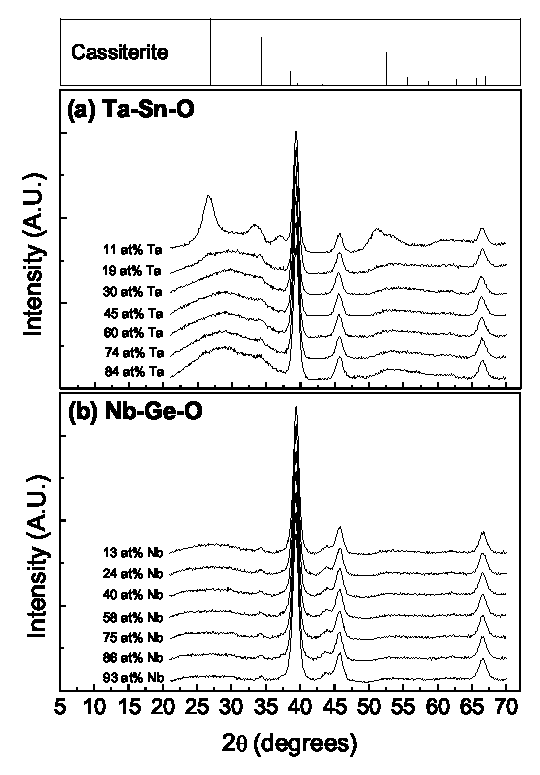
\includegraphics[width=0.5\linewidth]{chapter_6/tanbsngeox_wpdf.eps}
\caption{XRD spectra for (a) (Nb$_{2}$O$_{5}$)$_{1-x}$(GeO$_{2}$)$_{x}$ and (b) (Ta$_{2}$O$_{5}$)$_{1-x}$(SnO$_{2}$)$_{x}$ plotted for several cation compositions. The lack of any discernible diffraction peaks indicate that the (Nb$_{2}$O$_{5}$)$_{1-x}$(GeO$_{2}$)$_{x}$ is x-ray amorphous for the entire composition range probed. (Ta$_{2}$O$_{5}$)$_{1-x}$(SnO$_{2}$)$_{x}$ is x-ray amorphous for high Ta$_{2}$O$_{5}$ rich composition, but crystallizes at high SnO$_{2}$ concentrations.}
\label{fig:xrd2}
\end{figure}

\begin{figure}
\centering
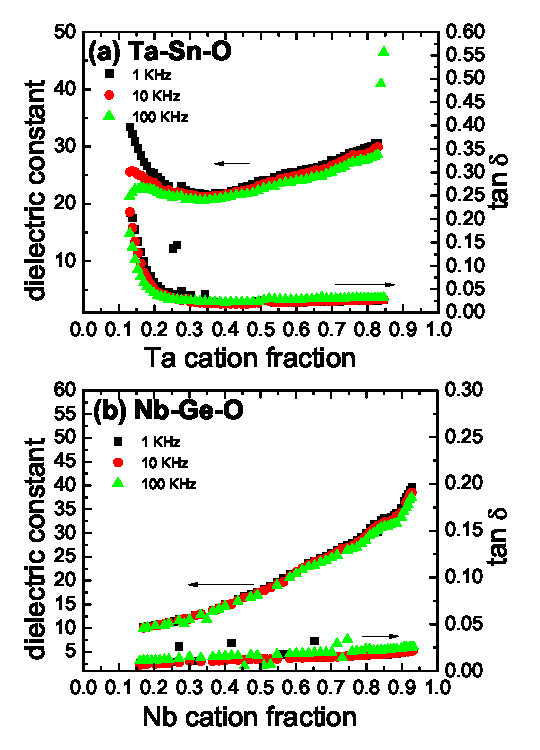
\includegraphics[width=0.5\linewidth]{chapter_6/eps_nbta.eps}
\caption{The dielectric constant and dissipation factor for (a) (Nb$_{2}$O$_{5}$)$_{1-x}$(GeO$_{2}$)$_{x}$ and (b) (Ta$_{2}$O$_{5}$)$_{1-x}$(SnO$_{2}$)$_{x}$ plotted as a function of composition. The  dielectric constant of (Nb$_{2}$O$_{5}$)$_{1-x}$(GeO$_{2}$)$_{x}$ shows a mostly linear dependence in $\varepsilon_{r}$ with composition, whereas (Ta$_{2}$O$_{5}$)$_{1-x}$(SnO$_{2}$)$_{x}$ shows a nondispersive and highly dispersive region.}
\label{fig:eps2}
\end{figure}

The sensitivity of the dopant concentration on the dielectric behavior of (Ta$_{2}$O$_{5}$)$_{1-x}$(SnO$_{2}$)$_{x}$ is shown in Figure \ref{fig:eps2}, where two distinct regions of dielectric behavior can be distinguished. For high Ta$_{2}$O$_{5}$ concentrations we observe a near linear dependence on the dielectric constant and in this region, the dissipation factor is also low ($\tan{\delta}<0.1$) indicating a high quality insulating film. Substitution of an aliovalent cation does not seem to promote a defect mediated transport mechanism such as hopping conductivity, as suggested by the low dissipation factor. Similarly, the substitution of ZrO$_{2}$ in Ta$_{2}$O$_{5}$ decreases the conductivity of Ta$_{2}$O$_{5}$ phase, the opposite of what is expected for a classical point defect model. \cite{Bredesen1988} The dielectric constant of the most Ta$_{2}$O$_{5}$ rich composition is around 27 at approximately 85 at\% Ta. Linearly extrapolating to pure Ta yields a dielectric constant of approximately $\varepsilon_{r} = 31$ which is enhanced over that of pure amorphous Ta$_{2}$O$_{5}$ ($\varepsilon_{r} = 22$), \cite{Barron2009} while extrapolation to pure SnO$_{2}$ gives $\varepsilon_{r} = 13$, consistent with literature values. \cite{albers1972} With further incorporation of SnO$_{2}$ $\varepsilon_{r}$ becomes dispersive, evidenced by a high dissipation factor ($\tan{\delta}>0.1$) and the highly frequency dependent nature of $\varepsilon_{r}$. This is not surprising since SnO$_{2}$ is a conductive oxide. \cite{singh2008} Diffraction patterns (Figure \ref{fig:xrd2}) show that the onset of crystallization correlates with the dispersive behavior, hence the dispersive nature of the film is likely caused by conduction within the SnO$_{2}$ rather than defects in Ta$_{2}$O$_{5}$. 

The dielectric constant of amorphous (Nb$_{2}$O$_{5}$)$_{1-x}$(GeO$_{2}$)$_{x}$ scales linearly with composition, with low dissipation factors, and shows no sign of dispersive behavior (Figure \ref{fig:eps2}). At an Nb cation concentration of 93\%  $\varepsilon_{r} \sim 42.5$, while extrapolation of $\varepsilon_{r}$ to pure Nb$_{2}$O$_{5}$ indicates a $\varepsilon_{r}$ for pure Nb$_{2}$O$_{5}$ $\sim 47-48$, which is comparable with $\varepsilon_{r}$ of fully oxidized Nb$_{2}$O$_{5}$ ($\varepsilon_{r}= 45-50$). \cite{Kukli1999,Pignolet1995}
Though the dielectric constant may not be dramatically enhanced over the end member, an insulating amorphous Nb$_{2}$O$_{5}$ thin film oxide may still be of technological interest, 
in particular since it is a  conductive oxide, \cite{Greener1961} that is sensitive to oxygen partial pressure during deposition. \cite{Pignolet1995} Because conductivity in Nb$_{2}$O$_{5}$ is inversely related to oxygen partial pressure it is often attributed to oxygen ion vacancies in Nb$_{2}$O$_{5}$  creating charge carriers that are thermally excited into  the conduction band. \cite{Greener1961} Doping aliovalent cations often create sites that enable dielectric relaxation via hopping. For instance, previous measurements on sintered (Nb$_{2}$O$_{5}$)$_{0.92}$(SiO$_{2}$)$_{0.08}$ bulk ceramic samples exhibited significant frequency dependent dielectric relaxation at room temperature. \cite{Choosuwan2003} Three distinct mechanisms were identified and the authors hypothesized that the relaxation species composed of hopping ions between the Nb and the substituted Si ion and the large dispersion is accompanied by a substantially higher dielectric constant ($\varepsilon_{r}\approx 125$ at room temperature). \cite{Choosuwan2003} 

\begin{figure}
\centering
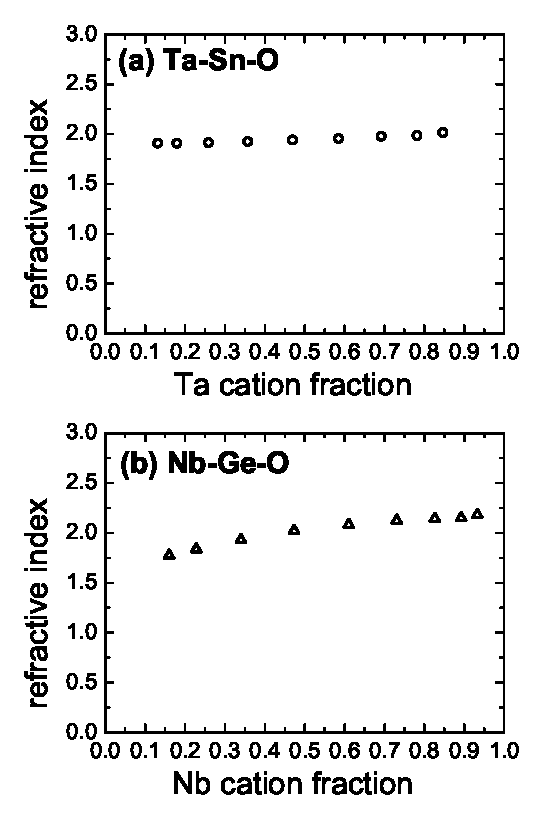
\includegraphics[width=0.5\linewidth]{chapter_6/n_tanb.eps}
\caption{Refractive index of (a) (Nb$_{2}$O$_{5}$)$_{1-x}$(GeO$_{2}$)$_{x}$ and (b) (Ta$_{2}$O$_{5}$)$_{1-x}$(SnO$_{2}$)$_{x}$ as function of Hf cation composition.}
\label{fig:ntanb}
\end{figure}

\begin{figure}
\centering
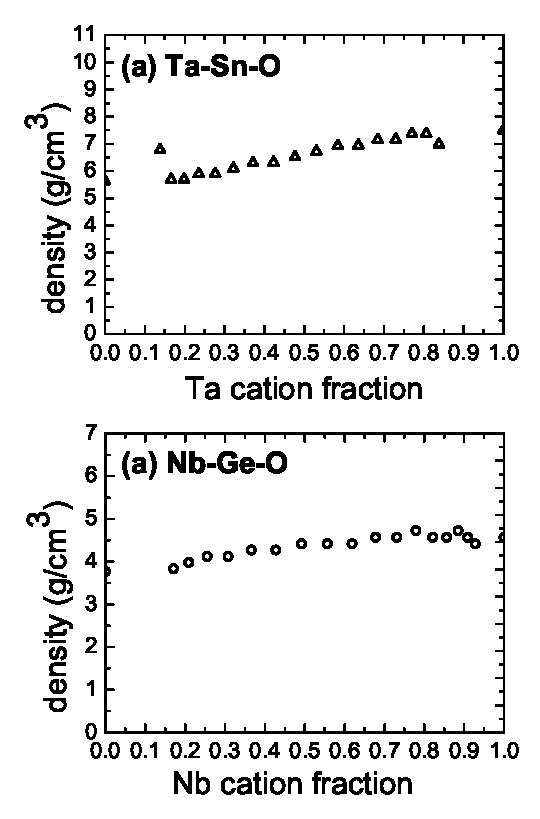
\includegraphics[width=0.5\linewidth]{chapter_6/tanbox_density.eps}
\caption{The density of (a) (Nb$_{2}$O$_{5}$)$_{1-x}$(GeO$_{2}$)$_{x}$ and (b) (Ta$_{2}$O$_{5}$)$_{1-x}$(SnO$_{2}$)$_{x}$ as function of Hf cation composition determined using XRR. The linear variation in density for (Nb$_{2}$O$_{5}$)$_{1-x}$(GeO$_{2}$)$_{x}$ as a function of composition reflects the amorphous nature of for all composition. (Ta$_{2}$O$_{5}$)$_{1-x}$(SnO$_{2}$)$_{x}$ densities also vary linearly except for the point where the film crystallizes.}
\label{fig:tanbden}
\end{figure}

Even with the introduction of GeO$_{2}$ into Nb$_{2}$O$_{5}$, the thin films exhibit low dissipation factors indicating the absence of a deleterious relaxation mechanism. Nonetheless, direct comparisons are difficult to make since the (Nb$_{2}$O$_{5}$)$_{0.92}$(SiO$_{2}$)$_{0.08}$ was a bulk crystalline ceramic, whereas our materials were amorphous thin films. Bulk crystalline ceramics contain grains and grain boundaries, which can contribute to several types of conduction mechanisms, which are absent in amorphous materials. 
     
Anomalous behaviors were not observed for the refractive indices for both systems (Figure \ref{fig:ntanb}) and the refractive index scales with composition. This trend is also reflected in the densities calculated from x-ray reflectivity (Figure \ref{fig:tanbden}). The density of the endmember values were also calculated directly from pure films deposited on to Si. Crystallization of the (Ta$_{2}$O$_{5}$)$_{1-x}$(SnO$_{2}$)$_{x}$ film at 0.14 Ta cation fraction causes the film density to jump to 6.78 g/cm$^{3}$ and is consistent with diffraction patterns and dielectric measurements. This makes it appear that the density is nonlinear, however the density of pure amorphous SnO$_{2}$ as seen in Figure \ref{fig:tanbden} is 5.62 g/cm$^{3}$ and is consistent with the linear trend. Since the refractive index reflects the electron density of the material increase in density should cause the refractive index to rise. Our refractive index measurements for (Ta$_{2}$O$_{5}$)$_{1-x}$(SnO$_{2}$)$_{x}$ do not go low enough in Ta cation fraction and thus we were not able to observe an increase in the refractive index. 

\section{Conclusion}

Using off-axis rf sputtering, we have studied the physical and dielectric properties of four pseudo-ternary oxides of varying composition: (HfO$_{2}$)$_{1-x}$(SiO$_{2}$)$_{x}$, (HfO$_{2}$)$_{1-x}$(GeO$_{2}$)$_{x}$, (Nb$_{2}$O$_{5}$)$_{1-x}$(GeO$_{2}$)$_{x}$, and (Ta$_{2}$O$_{5}$)$_{1-x}$(SnO$_{2}$)$_{x}$. Both (HfO$_{2}$)$_{1-x}$(SiO$_{2}$)$_{x}$ and (HfO$_{2}$)$_{1-x}$(GeO$_{2}$)$_{x}$ crystallized with increasing HfO$_{2}$ compositions and became amorphous with increasing concentrations of Si(Ge)O$_{2}$. The diffraction patterns of the two systems were similar, but the dielectric constants varied differently with composition. A clear peak in the dielectric constant can be observed in the (HfO$_{2}$)$_{1-x}$(SiO$_{2}$)$_{x}$ films, with a maximum dielectric constant of $\varepsilon_{r} = 28$ at 96 at$\%$ Hf, while the dielectric constant of (HfO$_{2}$)$_{1-x}$(GeO$_{2}$)$_{x}$ plateaus around $\varepsilon_{r} = 19$. Reflectivity measurements were consistent with the diffraction measurements and provided further detail into the amorphous-crystalline phase transition. The onset of crystallinity is slightly higher for the SiO$_{2}$ doped films; 80 at$\%$ Hf versus 70 at$\%$ for the GeO$_{2}$ doped films. In contrast to the dielectric constants, the refractive indices varies roughly linearly with composition.

(Ta$_{2}$O$_{5}$)$_{1-x}$(SnO$_{2}$)$_{x}$ was amorphous for SnO$_{2}$ poor compositions and crystallized into the cassiterite phase only for the most SnO$_{2}$ rich composition evaluated, and is indicated by a sudden increase in density. Increased dielectric dispersion and dissipation factor with increasing SnO$_{2}$ suggest that the film is becomes more conductive, where conduction is most likely through polycrystalline SnO$_{2}$ grains. Finally, (Nb$_{2}$O$_{5}$)$_{1-x}$(GeO$_{2}$)$_{x}$ was amorphous for all measured compositions and showed no anomalous features in the dielectric constant and refractive index. Not surprisingly, the density of the solid-solution changes linearly with composition. Doping low levels of GeO$_{2}$ into Nb$_{2}$O$_{5}$ resulted in a high quality dielectric and may be useful for applications requiring a high dielectric constant oxides.

% probably needs to be updated %
\section{Acknowledgments}
This work was supported by the U.S. Department of Energy under Grant No. DE-FG02-06ER06-15. This work was performed in part at the Cornell NanoScale Facility, a member of the National Nanotechnology Infrastructure Network, which is supported by the National Science Foundation under Grant No. ECS-0335765. Additionally, this work made use of the Cornell Center for Materials Research facilities with support from the National Science Foundation Materials Research Science and Engineering Center program under Grant No. DMR-0520404.

